% Chapter 1

\chapter{Introduction} % Main chapter title

\label{Chapter1} % For referencing the chapter elsewhere, use \ref{Chapter1} 

%----------------------------------------------------------------------------------------

% Define some commands to keep the formatting separated from the content 
\newcommand{\keyword}[1]{\textbf{#1}}
\newcommand{\tabhead}[1]{\textbf{#1}}
\newcommand{\code}[1]{\texttt{#1}}
\newcommand{\file}[1]{\texttt{\bfseries#1}}
\newcommand{\option}[1]{\texttt{\itshape#1}}

%----------------------------------------------------------------------------------------

\section{Project Description}

\section{Project Contents}
\subsection{Problem Description and Background}
\subsection{Overview of Related Literature}
\subsection{Research Question and Expected Outcomes}

\section{Aims and Objectives of Project}

\section{Procedures and Methods of Investigation}
\subsection{Research Paradigm and Methodology Used}
\subsection{Collection of Data}
\subsection{Development of Artefact}
\subsection{Integration with Other Projects}

\section{Approach to Project Management and Project Plan}
\subsection{Provisional Project Plan}

\begin{figure}[p]
\centering
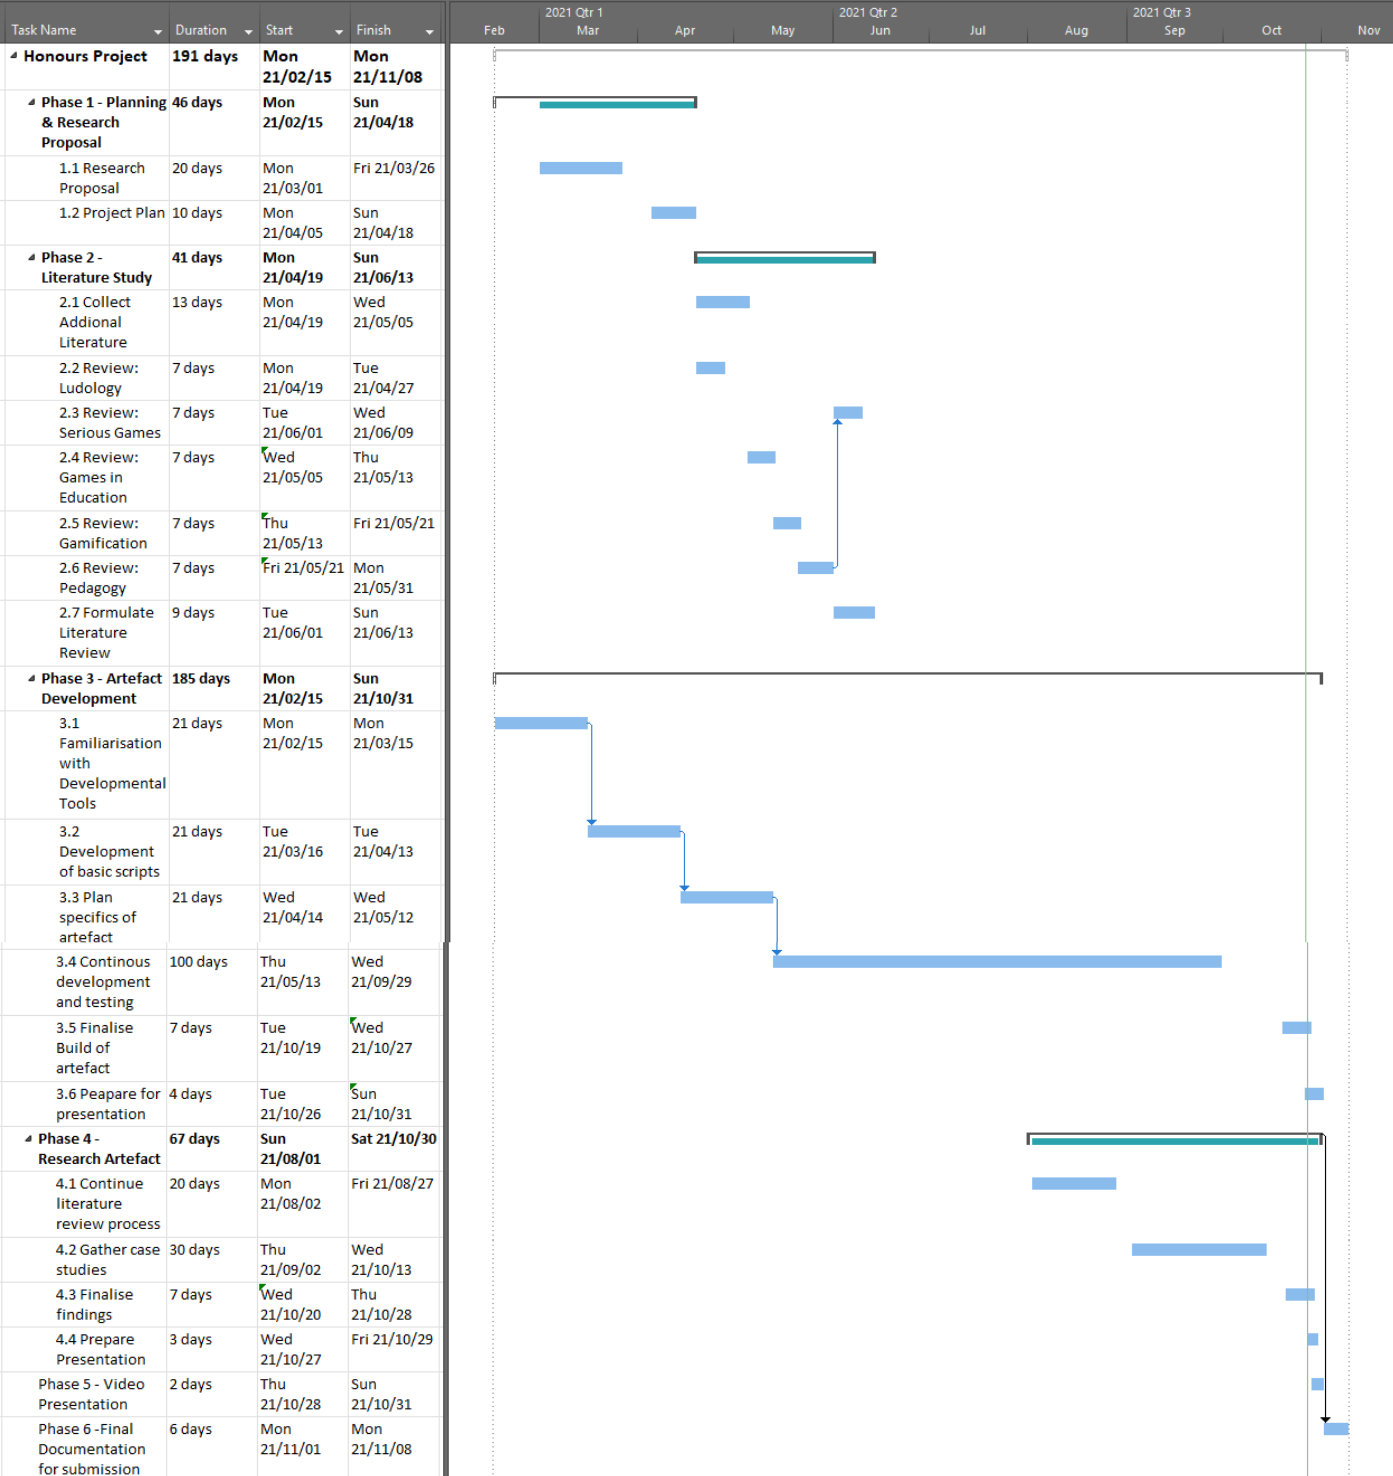
\includegraphics[scale=1.3]{gantt}
\caption{Provisional Project Plan}
\end{figure}

\subsection{Scope}
\subsection{Contributions of Each Group Member}

\section{Development Platform, Resources and Environments}
\subsection{Development Platform}
\subsection{Resources}
\subsection{Environments}

\section{Ethical Implications of Project}

\section{Provisional Chapter Division}

